\documentclass[1p]{elsarticle_modified}
%\bibliographystyle{elsarticle-num}

%\usepackage[colorlinks]{hyperref}
%\usepackage{abbrmath_seonhwa} %\Abb, \Ascr, \Acal ,\Abf, \Afrak
\usepackage{amsfonts}
\usepackage{amssymb}
\usepackage{amsmath}
\usepackage{amsthm}
\usepackage{scalefnt}
\usepackage{amsbsy}
\usepackage{kotex}
\usepackage{caption}
\usepackage{subfig}
\usepackage{color}
\usepackage{graphicx}
\usepackage{xcolor} %% white, black, red, green, blue, cyan, magenta, yellow
\usepackage{float}
\usepackage{setspace}
\usepackage{hyperref}

\usepackage{tikz}
\usetikzlibrary{arrows}

\usepackage{multirow}
\usepackage{array} % fixed length table
\usepackage{hhline}

%%%%%%%%%%%%%%%%%%%%%
\makeatletter
\renewcommand*\env@matrix[1][\arraystretch]{%
	\edef\arraystretch{#1}%
	\hskip -\arraycolsep
	\let\@ifnextchar\new@ifnextchar
	\array{*\c@MaxMatrixCols c}}
\makeatother %https://tex.stackexchange.com/questions/14071/how-can-i-increase-the-line-spacing-in-a-matrix
%%%%%%%%%%%%%%%

\usepackage[normalem]{ulem}

\newcommand{\msout}[1]{\ifmmode\text{\sout{\ensuremath{#1}}}\else\sout{#1}\fi}
%SOURCE: \msout is \stkout macro in https://tex.stackexchange.com/questions/20609/strikeout-in-math-mode

\newcommand{\cancel}[1]{
	\ifmmode
	{\color{red}\msout{#1}}
	\else
	{\color{red}\sout{#1}}
	\fi
}

\newcommand{\add}[1]{
	{\color{blue}\uwave{#1}}
}

\newcommand{\replace}[2]{
	\ifmmode
	{\color{red}\msout{#1}}{\color{blue}\uwave{#2}}
	\else
	{\color{red}\sout{#1}}{\color{blue}\uwave{#2}}
	\fi
}

\newcommand{\Sol}{\mathcal{S}} %segment
\newcommand{\D}{D} %diagram
\newcommand{\A}{\mathcal{A}} %arc


%%%%%%%%%%%%%%%%%%%%%%%%%%%%%5 test

\def\sl{\operatorname{\textup{SL}}(2,\Cbb)}
\def\psl{\operatorname{\textup{PSL}}(2,\Cbb)}
\def\quan{\mkern 1mu \triangleright \mkern 1mu}

\theoremstyle{definition}
\newtheorem{thm}{Theorem}[section]
\newtheorem{prop}[thm]{Proposition}
\newtheorem{lem}[thm]{Lemma}
\newtheorem{ques}[thm]{Question}
\newtheorem{cor}[thm]{Corollary}
\newtheorem{defn}[thm]{Definition}
\newtheorem{exam}[thm]{Example}
\newtheorem{rmk}[thm]{Remark}
\newtheorem{alg}[thm]{Algorithm}

\newcommand{\I}{\sqrt{-1}}
\begin{document}

%\begin{frontmatter}
%
%\title{Boundary parabolic representations of knots up to 8 crossings}
%
%%% Group authors per affiliation:
%\author{Yunhi Cho} 
%\address{Department of Mathematics, University of Seoul, Seoul, Korea}
%\ead{yhcho@uos.ac.kr}
%
%
%\author{Seonhwa Kim} %\fnref{s_kim}}
%\address{Center for Geometry and Physics, Institute for Basic Science, Pohang, 37673, Korea}
%\ead{ryeona17@ibs.re.kr}
%
%\author{Hyuk Kim}
%\address{Department of Mathematical Sciences, Seoul National University, Seoul 08826, Korea}
%\ead{hyukkim@snu.ac.kr}
%
%\author{Seokbeom Yoon}
%\address{Department of Mathematical Sciences, Seoul National University, Seoul, 08826,  Korea}
%\ead{sbyoon15@snu.ac.kr}
%
%\begin{abstract}
%We find all boundary parabolic representation of knots up to 8 crossings.
%
%\end{abstract}
%\begin{keyword}
%    \MSC[2010] 57M25 
%\end{keyword}
%
%\end{frontmatter}

%\linenumbers
%\tableofcontents
%
\newcommand\colored[1]{\textcolor{white}{\rule[-0.35ex]{0.8em}{1.4ex}}\kern-0.8em\color{red} #1}%
%\newcommand\colored[1]{\textcolor{white}{ #1}\kern-2.17ex	\textcolor{white}{ #1}\kern-1.81ex	\textcolor{white}{ #1}\kern-2.15ex\color{red}#1	}

{\Large $\underline{12a_{0941}~(K12a_{0941})}$}

\setlength{\tabcolsep}{10pt}
\renewcommand{\arraystretch}{1.6}
\vspace{1cm}\begin{tabular}{m{100pt}>{\centering\arraybackslash}m{274pt}}
\multirow{5}{120pt}{
	\centering
	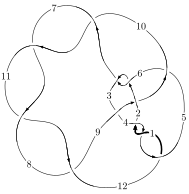
\includegraphics[width=112pt]{../../../GIT/diagram.site/Diagrams/png/1742_12a_0941.png}\\
\ \ \ A knot diagram\footnotemark}&
\allowdisplaybreaks
\textbf{Linearized knot diagam} \\
\cline{2-2}
 &
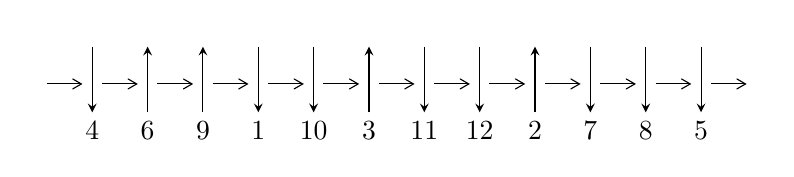
\begin{tikzpicture}[x=20pt, y=17pt]
	% nodes
	\node (C0) at (0, 0) {};
	\node (C1) at (1, 0) {};
	\node (C1U) at (1, +1) {};
	\node (C1D) at (1, -1) {4};

	\node (C2) at (2, 0) {};
	\node (C2U) at (2, +1) {};
	\node (C2D) at (2, -1) {6};

	\node (C3) at (3, 0) {};
	\node (C3U) at (3, +1) {};
	\node (C3D) at (3, -1) {9};

	\node (C4) at (4, 0) {};
	\node (C4U) at (4, +1) {};
	\node (C4D) at (4, -1) {1};

	\node (C5) at (5, 0) {};
	\node (C5U) at (5, +1) {};
	\node (C5D) at (5, -1) {10};

	\node (C6) at (6, 0) {};
	\node (C6U) at (6, +1) {};
	\node (C6D) at (6, -1) {3};

	\node (C7) at (7, 0) {};
	\node (C7U) at (7, +1) {};
	\node (C7D) at (7, -1) {11};

	\node (C8) at (8, 0) {};
	\node (C8U) at (8, +1) {};
	\node (C8D) at (8, -1) {12};

	\node (C9) at (9, 0) {};
	\node (C9U) at (9, +1) {};
	\node (C9D) at (9, -1) {2};

	\node (C10) at (10, 0) {};
	\node (C10U) at (10, +1) {};
	\node (C10D) at (10, -1) {7};

	\node (C11) at (11, 0) {};
	\node (C11U) at (11, +1) {};
	\node (C11D) at (11, -1) {8};

	\node (C12) at (12, 0) {};
	\node (C12U) at (12, +1) {};
	\node (C12D) at (12, -1) {5};
	\node (C13) at (13, 0) {};

	% arrows
	\draw[->,>={angle 60}]
	(C0) edge (C1) (C1) edge (C2) (C2) edge (C3) (C3) edge (C4) (C4) edge (C5) (C5) edge (C6) (C6) edge (C7) (C7) edge (C8) (C8) edge (C9) (C9) edge (C10) (C10) edge (C11) (C11) edge (C12) (C12) edge (C13) ;	\draw[->,>=stealth]
	(C1U) edge (C1D) (C2D) edge (C2U) (C3D) edge (C3U) (C4U) edge (C4D) (C5U) edge (C5D) (C6D) edge (C6U) (C7U) edge (C7D) (C8U) edge (C8D) (C9D) edge (C9U) (C10U) edge (C10D) (C11U) edge (C11D) (C12U) edge (C12D) ;
	\end{tikzpicture} \\
\hhline{~~} \\& 
\textbf{Solving Sequence} \\ \cline{2-2} 
 &
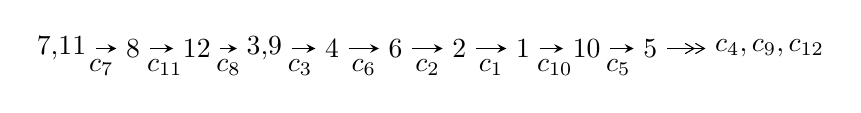
\begin{tikzpicture}[x=23pt, y=7pt]
	% node
	\node (A0) at (-1/8, 0) {7,11};
	\node (A1) at (1, 0) {8};
	\node (A2) at (2, 0) {12};
	\node (A3) at (49/16, 0) {3,9};
	\node (A4) at (33/8, 0) {4};
	\node (A5) at (41/8, 0) {6};
	\node (A6) at (49/8, 0) {2};
	\node (A7) at (57/8, 0) {1};
	\node (A8) at (65/8, 0) {10};
	\node (A9) at (73/8, 0) {5};
	\node (C1) at (1/2, -1) {$c_{7}$};
	\node (C2) at (3/2, -1) {$c_{11}$};
	\node (C3) at (5/2, -1) {$c_{8}$};
	\node (C4) at (29/8, -1) {$c_{3}$};
	\node (C5) at (37/8, -1) {$c_{6}$};
	\node (C6) at (45/8, -1) {$c_{2}$};
	\node (C7) at (53/8, -1) {$c_{1}$};
	\node (C8) at (61/8, -1) {$c_{10}$};
	\node (C9) at (69/8, -1) {$c_{5}$};
	\node (A10) at (11, 0) {$c_{4},c_{9},c_{12}$};

	% edge
	\draw[->,>=stealth]	
	(A0) edge (A1) (A1) edge (A2) (A2) edge (A3) (A3) edge (A4) (A4) edge (A5) (A5) edge (A6) (A6) edge (A7) (A7) edge (A8) (A8) edge (A9) ;
	\draw[->>,>={angle 60}]	
	(A9) edge (A10);
\end{tikzpicture} \\ 

\end{tabular} \\

\footnotetext{
The image of knot diagram is generated by the software ``\textbf{Draw programme}" developed by Andrew Bartholomew(\url{http://www.layer8.co.uk/maths/draw/index.htm\#Running-draw}), where we modified some parts for our purpose(\url{https://github.com/CATsTAILs/LinksPainter}).
}\phantom \\ \newline 
\centering \textbf{Ideals for irreducible components\footnotemark of $X_{\text{par}}$} 
 
\begin{align*}
I^u_{1}&=\langle 
-1.42999\times10^{69} u^{73}+6.42092\times10^{69} u^{72}+\cdots+1.65516\times10^{69} b+1.02869\times10^{70},\\
\phantom{I^u_{1}}&\phantom{= \langle  }-5.07268\times10^{70} u^{73}+2.49297\times10^{71} u^{72}+\cdots+1.48964\times10^{70} a+6.53143\times10^{71},\;u^{74}-6 u^{73}+\cdots-5 u+9\rangle \\
I^u_{2}&=\langle 
5 b-3 a-1,\;3 a^2-3 a+7,\;u^2+u-1\rangle \\
I^u_{3}&=\langle 
b+1,\;a^2+2 a+3,\;u-1\rangle \\
I^u_{4}&=\langle 
b-1,\;a-1,\;u-1\rangle \\
\\
\end{align*}
\raggedright * 4 irreducible components of $\dim_{\mathbb{C}}=0$, with total 81 representations.\\
\footnotetext{All coefficients of polynomials are rational numbers. But the coefficients are sometimes approximated in decimal forms when there is not enough margin.}
\newpage
\renewcommand{\arraystretch}{1}
\centering \section*{I. $I^u_{1}= \langle -1.43\times10^{69} u^{73}+6.42\times10^{69} u^{72}+\cdots+1.66\times10^{69} b+1.03\times10^{70},\;-5.07\times10^{70} u^{73}+2.49\times10^{71} u^{72}+\cdots+1.49\times10^{70} a+6.53\times10^{71},\;u^{74}-6 u^{73}+\cdots-5 u+9 \rangle$}
\flushleft \textbf{(i) Arc colorings}\\
\begin{tabular}{m{7pt} m{180pt} m{7pt} m{180pt} }
\flushright $a_{7}=$&$\begin{pmatrix}1\\0\end{pmatrix}$ \\
\flushright $a_{11}=$&$\begin{pmatrix}0\\u\end{pmatrix}$ \\
\flushright $a_{8}=$&$\begin{pmatrix}1\\u^2\end{pmatrix}$ \\
\flushright $a_{12}=$&$\begin{pmatrix}- u\\- u^3+u\end{pmatrix}$ \\
\flushright $a_{3}=$&$\begin{pmatrix}3.40530 u^{73}-16.7354 u^{72}+\cdots-59.8211 u-43.8456\\0.863958 u^{73}-3.87934 u^{72}+\cdots-2.16199 u-6.21506\end{pmatrix}$ \\
\flushright $a_{9}=$&$\begin{pmatrix}- u^2+1\\- u^4+2 u^2\end{pmatrix}$ \\
\flushright $a_{4}=$&$\begin{pmatrix}0.875009 u^{73}-4.53530 u^{72}+\cdots-39.7678 u-20.7618\\1.73096 u^{73}-7.25329 u^{72}+\cdots+3.74996 u-8.00046\end{pmatrix}$ \\
\flushright $a_{6}=$&$\begin{pmatrix}4.28594 u^{73}-19.7999 u^{72}+\cdots-55.8776 u-44.5013\\6.03936 u^{73}-26.3358 u^{72}+\cdots-2.69922 u-34.6744\end{pmatrix}$ \\
\flushright $a_{2}=$&$\begin{pmatrix}11.7060 u^{73}-52.9235 u^{72}+\cdots-13.7202 u-74.9192\\8.41966 u^{73}-37.8131 u^{72}+\cdots-2.40204 u-50.4595\end{pmatrix}$ \\
\flushright $a_{1}=$&$\begin{pmatrix}5.78714 u^{73}-29.6988 u^{72}+\cdots-74.5556 u-72.6750\\0.856731 u^{73}-2.06038 u^{72}+\cdots+50.8868 u+18.9089\end{pmatrix}$ \\
\flushright $a_{10}=$&$\begin{pmatrix}u\\u\end{pmatrix}$ \\
\flushright $a_{5}=$&$\begin{pmatrix}10.6776 u^{73}-48.4916 u^{72}+\cdots-51.7357 u-80.3621\\12.4311 u^{73}-55.0275 u^{72}+\cdots+1.44267 u-70.5352\end{pmatrix}$\\&\end{tabular}
\flushleft \textbf{(ii) Obstruction class $= -1$}\\~\\
\flushleft \textbf{(iii) Cusp Shapes $= 5.31177 u^{73}-18.4801 u^{72}+\cdots+92.2939 u+19.8328$}\\~\\
\newpage\renewcommand{\arraystretch}{1}
\flushleft \textbf{(iv) u-Polynomials at the component}\newline \\
\begin{tabular}{m{50pt}|m{274pt}}
Crossings & \hspace{64pt}u-Polynomials at each crossing \\
\hline $$\begin{aligned}c_{1},c_{4},c_{12}\end{aligned}$$&$\begin{aligned}
&u^{74}-3 u^{73}+\cdots-12 u+2
\end{aligned}$\\
\hline $$\begin{aligned}c_{2},c_{6}\end{aligned}$$&$\begin{aligned}
&u^{74}-4 u^{73}+\cdots-5 u-3
\end{aligned}$\\
\hline $$\begin{aligned}c_{3}\end{aligned}$$&$\begin{aligned}
&9(9 u^{74}+30 u^{73}+\cdots-18775 u+11591)
\end{aligned}$\\
\hline $$\begin{aligned}c_{5}\end{aligned}$$&$\begin{aligned}
&9(9 u^{74}-39 u^{73}+\cdots+17840 u+853)
\end{aligned}$\\
\hline $$\begin{aligned}c_{7},c_{8},c_{10}\\c_{11}\end{aligned}$$&$\begin{aligned}
&u^{74}+6 u^{73}+\cdots+5 u+9
\end{aligned}$\\
\hline $$\begin{aligned}c_{9}\end{aligned}$$&$\begin{aligned}
&u^{74}+2 u^{73}+\cdots+576 u-432
\end{aligned}$\\
\hline
\end{tabular}\\~\\
\newpage\renewcommand{\arraystretch}{1}
\flushleft \textbf{(v) Riley Polynomials at the component}\newline \\
\begin{tabular}{m{50pt}|m{274pt}}
Crossings & \hspace{64pt}Riley Polynomials at each crossing \\
\hline $$\begin{aligned}c_{1},c_{4},c_{12}\end{aligned}$$&$\begin{aligned}
&y^{74}+69 y^{73}+\cdots-48 y+4
\end{aligned}$\\
\hline $$\begin{aligned}c_{2},c_{6}\end{aligned}$$&$\begin{aligned}
&y^{74}-38 y^{73}+\cdots-775 y+9
\end{aligned}$\\
\hline $$\begin{aligned}c_{3}\end{aligned}$$&$\begin{aligned}
&81(81 y^{74}-2970 y^{73}+\cdots-1.79556\times10^{9} y+1.34351\times10^{8})
\end{aligned}$\\
\hline $$\begin{aligned}c_{5}\end{aligned}$$&$\begin{aligned}
&81(81 y^{74}-729 y^{73}+\cdots-2.92408\times10^{8} y+727609)
\end{aligned}$\\
\hline $$\begin{aligned}c_{7},c_{8},c_{10}\\c_{11}\end{aligned}$$&$\begin{aligned}
&y^{74}-86 y^{73}+\cdots-655 y+81
\end{aligned}$\\
\hline $$\begin{aligned}c_{9}\end{aligned}$$&$\begin{aligned}
&y^{74}-28 y^{73}+\cdots-2104704 y+186624
\end{aligned}$\\
\hline
\end{tabular}\\~\\
\newpage\flushleft \textbf{(vi) Complex Volumes and Cusp Shapes}
$$\begin{array}{c|c|c}  
\text{Solutions to }I^u_{1}& \I (\text{vol} + \sqrt{-1}CS) & \text{Cusp shape}\\
 \hline 
\begin{aligned}
u &= -0.780489 + 0.653369 I \\
a &= \phantom{-}0.48251 - 1.51030 I \\
b &= -1.252830 - 0.542624 I\end{aligned}
 & \phantom{-}7.3329 + 12.3570 I & \phantom{-0.000000 } 0 \\ \hline\begin{aligned}
u &= -0.780489 - 0.653369 I \\
a &= \phantom{-}0.48251 + 1.51030 I \\
b &= -1.252830 + 0.542624 I\end{aligned}
 & \phantom{-}7.3329 - 12.3570 I & \phantom{-0.000000 } 0 \\ \hline\begin{aligned}
u &= \phantom{-}0.926260 + 0.427283 I \\
a &= \phantom{-}0.703366 + 0.640455 I \\
b &= -0.349481 + 0.290897 I\end{aligned}
 & \phantom{-}2.66093 - 0.33343 I & \phantom{-0.000000 } 0 \\ \hline\begin{aligned}
u &= \phantom{-}0.926260 - 0.427283 I \\
a &= \phantom{-}0.703366 - 0.640455 I \\
b &= -0.349481 - 0.290897 I\end{aligned}
 & \phantom{-}2.66093 + 0.33343 I & \phantom{-0.000000 } 0 \\ \hline\begin{aligned}
u &= -0.766830 + 0.541355 I \\
a &= -0.35452 + 1.57607 I \\
b &= \phantom{-}1.236780 + 0.551197 I\end{aligned}
 & \phantom{-}1.12893 + 8.60971 I & \phantom{-0.000000 } 0 \\ \hline\begin{aligned}
u &= -0.766830 - 0.541355 I \\
a &= -0.35452 - 1.57607 I \\
b &= \phantom{-}1.236780 - 0.551197 I\end{aligned}
 & \phantom{-}1.12893 - 8.60971 I & \phantom{-0.000000 } 0 \\ \hline\begin{aligned}
u &= \phantom{-}0.722917 + 0.572819 I \\
a &= \phantom{-}0.197853 + 0.324737 I \\
b &= -0.555314 - 0.341105 I\end{aligned}
 & \phantom{-}2.44985 - 0.53730 I & \phantom{-0.000000 } 0 \\ \hline\begin{aligned}
u &= \phantom{-}0.722917 - 0.572819 I \\
a &= \phantom{-}0.197853 - 0.324737 I \\
b &= -0.555314 + 0.341105 I\end{aligned}
 & \phantom{-}2.44985 + 0.53730 I & \phantom{-0.000000 } 0 \\ \hline\begin{aligned}
u &= -0.745115 + 0.507872 I \\
a &= -0.505661 + 0.814141 I \\
b &= -0.133191 + 0.959429 I\end{aligned}
 & \phantom{-}3.89877 + 6.97858 I & \phantom{-0.000000 } 0 \\ \hline\begin{aligned}
u &= -0.745115 - 0.507872 I \\
a &= -0.505661 - 0.814141 I \\
b &= -0.133191 - 0.959429 I\end{aligned}
 & \phantom{-}3.89877 - 6.97858 I & \phantom{-0.000000 } 0\\
 \hline 
 \end{array}$$\newpage$$\begin{array}{c|c|c}  
\text{Solutions to }I^u_{1}& \I (\text{vol} + \sqrt{-1}CS) & \text{Cusp shape}\\
 \hline 
\begin{aligned}
u &= \phantom{-}1.058370 + 0.376551 I \\
a &= \phantom{-}0.390460 - 0.275743 I \\
b &= \phantom{-}0.938072 + 0.240382 I\end{aligned}
 & -0.571733 + 0.687366 I & \phantom{-0.000000 } 0 \\ \hline\begin{aligned}
u &= \phantom{-}1.058370 - 0.376551 I \\
a &= \phantom{-}0.390460 + 0.275743 I \\
b &= \phantom{-}0.938072 - 0.240382 I\end{aligned}
 & -0.571733 - 0.687366 I & \phantom{-0.000000 } 0 \\ \hline\begin{aligned}
u &= -0.209015 + 0.842113 I \\
a &= \phantom{-}0.613156 - 0.007223 I \\
b &= -1.188410 + 0.452211 I\end{aligned}
 & \phantom{-}9.07024 - 7.42311 I & \phantom{-0.000000 } 0 \\ \hline\begin{aligned}
u &= -0.209015 - 0.842113 I \\
a &= \phantom{-}0.613156 + 0.007223 I \\
b &= -1.188410 - 0.452211 I\end{aligned}
 & \phantom{-}9.07024 + 7.42311 I & \phantom{-0.000000 } 0 \\ \hline\begin{aligned}
u &= \phantom{-}0.456967 + 0.724258 I \\
a &= \phantom{-}1.005020 + 0.543237 I \\
b &= -0.876049 + 0.413421 I\end{aligned}
 & \phantom{-}3.31198 - 4.04047 I & \phantom{-0.000000 } 0 \\ \hline\begin{aligned}
u &= \phantom{-}0.456967 - 0.724258 I \\
a &= \phantom{-}1.005020 - 0.543237 I \\
b &= -0.876049 - 0.413421 I\end{aligned}
 & \phantom{-}3.31198 + 4.04047 I & \phantom{-0.000000 } 0 \\ \hline\begin{aligned}
u &= \phantom{-}0.610837 + 0.528728 I \\
a &= -0.906740 - 0.910567 I \\
b &= \phantom{-}0.766366 - 0.275897 I\end{aligned}
 & -0.93403 - 1.81717 I & -10.28717 + 6.80364 I \\ \hline\begin{aligned}
u &= \phantom{-}0.610837 - 0.528728 I \\
a &= -0.906740 + 0.910567 I \\
b &= \phantom{-}0.766366 + 0.275897 I\end{aligned}
 & -0.93403 + 1.81717 I & -10.28717 - 6.80364 I \\ \hline\begin{aligned}
u &= -0.654850 + 0.418140 I \\
a &= \phantom{-}0.18276 - 1.79134 I \\
b &= -1.202110 - 0.564951 I\end{aligned}
 & \phantom{-}1.73943 + 3.84518 I & -2.69909 - 5.52948 I \\ \hline\begin{aligned}
u &= -0.654850 - 0.418140 I \\
a &= \phantom{-}0.18276 + 1.79134 I \\
b &= -1.202110 + 0.564951 I\end{aligned}
 & \phantom{-}1.73943 - 3.84518 I & -2.69909 + 5.52948 I\\
 \hline 
 \end{array}$$\newpage$$\begin{array}{c|c|c}  
\text{Solutions to }I^u_{1}& \I (\text{vol} + \sqrt{-1}CS) & \text{Cusp shape}\\
 \hline 
\begin{aligned}
u &= -0.689051 + 0.317719 I \\
a &= \phantom{-}0.557656 - 1.039220 I \\
b &= \phantom{-}0.192843 - 0.984641 I\end{aligned}
 & -2.13148 + 3.14846 I & -7.44124 - 8.73816 I \\ \hline\begin{aligned}
u &= -0.689051 - 0.317719 I \\
a &= \phantom{-}0.557656 + 1.039220 I \\
b &= \phantom{-}0.192843 + 0.984641 I\end{aligned}
 & -2.13148 - 3.14846 I & -7.44124 + 8.73816 I \\ \hline\begin{aligned}
u &= \phantom{-}0.743515\phantom{ +0.000000I} \\
a &= -0.472726\phantom{ +0.000000I} \\
b &= \phantom{-}0.111724\phantom{ +0.000000I}\end{aligned}
 & -1.29107\phantom{ +0.000000I} & -8.03060\phantom{ +0.000000I} \\ \hline\begin{aligned}
u &= -0.129068 + 0.704485 I \\
a &= -0.719921 + 0.160016 I \\
b &= \phantom{-}1.159780 - 0.397161 I\end{aligned}
 & \phantom{-}3.03854 - 4.45334 I & -0.92150 + 5.94186 I \\ \hline\begin{aligned}
u &= -0.129068 - 0.704485 I \\
a &= -0.719921 - 0.160016 I \\
b &= \phantom{-}1.159780 + 0.397161 I\end{aligned}
 & \phantom{-}3.03854 + 4.45334 I & -0.92150 - 5.94186 I \\ \hline\begin{aligned}
u &= -0.506904 + 0.477161 I \\
a &= -0.0436695 + 0.0957579 I \\
b &= \phantom{-}1.324910 - 0.354848 I\end{aligned}
 & \phantom{-}8.65870 + 2.36010 I & \phantom{-}2.52056 - 4.62942 I \\ \hline\begin{aligned}
u &= -0.506904 - 0.477161 I \\
a &= -0.0436695 - 0.0957579 I \\
b &= \phantom{-}1.324910 + 0.354848 I\end{aligned}
 & \phantom{-}8.65870 - 2.36010 I & \phantom{-}2.52056 + 4.62942 I \\ \hline\begin{aligned}
u &= \phantom{-}1.257500 + 0.465420 I \\
a &= -0.340473 + 0.018485 I \\
b &= -1.047160 - 0.375595 I\end{aligned}
 & \phantom{-}4.58375 + 2.82748 I & \phantom{-0.000000 } 0 \\ \hline\begin{aligned}
u &= \phantom{-}1.257500 - 0.465420 I \\
a &= -0.340473 - 0.018485 I \\
b &= -1.047160 + 0.375595 I\end{aligned}
 & \phantom{-}4.58375 - 2.82748 I & \phantom{-0.000000 } 0 \\ \hline\begin{aligned}
u &= -0.113465 + 0.635641 I \\
a &= \phantom{-}0.809632 - 0.222688 I \\
b &= -0.032593 - 0.706254 I\end{aligned}
 & \phantom{-}5.75300 - 3.13005 I & -0.47310 + 1.96058 I\\
 \hline 
 \end{array}$$\newpage$$\begin{array}{c|c|c}  
\text{Solutions to }I^u_{1}& \I (\text{vol} + \sqrt{-1}CS) & \text{Cusp shape}\\
 \hline 
\begin{aligned}
u &= -0.113465 - 0.635641 I \\
a &= \phantom{-}0.809632 + 0.222688 I \\
b &= -0.032593 + 0.706254 I\end{aligned}
 & \phantom{-}5.75300 + 3.13005 I & -0.47310 - 1.96058 I \\ \hline\begin{aligned}
u &= \phantom{-}0.623383 + 0.158653 I \\
a &= -0.32416 + 3.34499 I \\
b &= -0.921135 + 0.058648 I\end{aligned}
 & \phantom{-}0.485464 - 0.382772 I & \phantom{-}9.7234 - 10.9570 I \\ \hline\begin{aligned}
u &= \phantom{-}0.623383 - 0.158653 I \\
a &= -0.32416 - 3.34499 I \\
b &= -0.921135 - 0.058648 I\end{aligned}
 & \phantom{-}0.485464 + 0.382772 I & \phantom{-}9.7234 + 10.9570 I \\ \hline\begin{aligned}
u &= -0.416679 + 0.480285 I \\
a &= -0.52731 + 2.30548 I \\
b &= \phantom{-}1.149740 + 0.482784 I\end{aligned}
 & \phantom{-}8.91952 + 1.00599 I & \phantom{-}3.16723 - 4.49529 I \\ \hline\begin{aligned}
u &= -0.416679 - 0.480285 I \\
a &= -0.52731 - 2.30548 I \\
b &= \phantom{-}1.149740 - 0.482784 I\end{aligned}
 & \phantom{-}8.91952 - 1.00599 I & \phantom{-}3.16723 + 4.49529 I \\ \hline\begin{aligned}
u &= -0.519626 + 0.103037 I \\
a &= -0.91143 + 1.58062 I \\
b &= -0.521721 + 0.994680 I\end{aligned}
 & -0.77301 - 1.82140 I & \phantom{-}7.86976 - 8.66716 I \\ \hline\begin{aligned}
u &= -0.519626 - 0.103037 I \\
a &= -0.91143 - 1.58062 I \\
b &= -0.521721 - 0.994680 I\end{aligned}
 & -0.77301 + 1.82140 I & \phantom{-}7.86976 + 8.66716 I \\ \hline\begin{aligned}
u &= \phantom{-}0.505606 + 0.052276 I \\
a &= -6.60990 + 5.71947 I \\
b &= \phantom{-}1.027770 + 0.072612 I\end{aligned}
 & \phantom{-}5.81053 - 0.10803 I & -4.98191 - 7.31698 I \\ \hline\begin{aligned}
u &= \phantom{-}0.505606 - 0.052276 I \\
a &= -6.60990 - 5.71947 I \\
b &= \phantom{-}1.027770 - 0.072612 I\end{aligned}
 & \phantom{-}5.81053 + 0.10803 I & -4.98191 + 7.31698 I \\ \hline\begin{aligned}
u &= \phantom{-}1.49577\phantom{ +0.000000I} \\
a &= -0.878655\phantom{ +0.000000I} \\
b &= -1.51662\phantom{ +0.000000I}\end{aligned}
 & -2.46559\phantom{ +0.000000I} & \phantom{-0.000000 } 0\\
 \hline 
 \end{array}$$\newpage$$\begin{array}{c|c|c}  
\text{Solutions to }I^u_{1}& \I (\text{vol} + \sqrt{-1}CS) & \text{Cusp shape}\\
 \hline 
\begin{aligned}
u &= \phantom{-}1.49843 + 0.08478 I \\
a &= \phantom{-}0.84047 - 1.98778 I \\
b &= \phantom{-}0.974646 - 0.722897 I\end{aligned}
 & \phantom{-}2.64300 - 2.84023 I & \phantom{-0.000000 } 0 \\ \hline\begin{aligned}
u &= \phantom{-}1.49843 - 0.08478 I \\
a &= \phantom{-}0.84047 + 1.98778 I \\
b &= \phantom{-}0.974646 + 0.722897 I\end{aligned}
 & \phantom{-}2.64300 + 2.84023 I & \phantom{-0.000000 } 0 \\ \hline\begin{aligned}
u &= -0.222562 + 0.436276 I \\
a &= \phantom{-}0.363985 - 0.713608 I \\
b &= -1.218890 + 0.287656 I\end{aligned}
 & \phantom{-}2.97702 - 0.79262 I & \phantom{-}0.91124 - 2.75524 I \\ \hline\begin{aligned}
u &= -0.222562 - 0.436276 I \\
a &= \phantom{-}0.363985 + 0.713608 I \\
b &= -1.218890 - 0.287656 I\end{aligned}
 & \phantom{-}2.97702 + 0.79262 I & \phantom{-}0.91124 + 2.75524 I \\ \hline\begin{aligned}
u &= \phantom{-}1.52960 + 0.11352 I \\
a &= \phantom{-}0.789714 + 0.238208 I \\
b &= \phantom{-}1.48319 + 0.25429 I\end{aligned}
 & \phantom{-}1.87547 - 4.40034 I & \phantom{-0.000000 } 0 \\ \hline\begin{aligned}
u &= \phantom{-}1.52960 - 0.11352 I \\
a &= \phantom{-}0.789714 - 0.238208 I \\
b &= \phantom{-}1.48319 - 0.25429 I\end{aligned}
 & \phantom{-}1.87547 + 4.40034 I & \phantom{-0.000000 } 0 \\ \hline\begin{aligned}
u &= -1.54223 + 0.22663 I \\
a &= \phantom{-}0.121615 - 1.194980 I \\
b &= -1.068200 - 0.517925 I\end{aligned}
 & -3.32651 + 7.47374 I & \phantom{-0.000000 } 0 \\ \hline\begin{aligned}
u &= -1.54223 - 0.22663 I \\
a &= \phantom{-}0.121615 + 1.194980 I \\
b &= -1.068200 + 0.517925 I\end{aligned}
 & -3.32651 - 7.47374 I & \phantom{-0.000000 } 0 \\ \hline\begin{aligned}
u &= -1.56341 + 0.01756 I \\
a &= -0.80268 - 1.74739 I \\
b &= \phantom{-}1.121450 - 0.237964 I\end{aligned}
 & -1.346100 + 0.385297 I & \phantom{-0.000000 } 0 \\ \hline\begin{aligned}
u &= -1.56341 - 0.01756 I \\
a &= -0.80268 + 1.74739 I \\
b &= \phantom{-}1.121450 + 0.237964 I\end{aligned}
 & -1.346100 - 0.385297 I & \phantom{-0.000000 } 0\\
 \hline 
 \end{array}$$\newpage$$\begin{array}{c|c|c}  
\text{Solutions to }I^u_{1}& \I (\text{vol} + \sqrt{-1}CS) & \text{Cusp shape}\\
 \hline 
\begin{aligned}
u &= \phantom{-}1.57344 + 0.03838 I \\
a &= -0.73507 - 1.79325 I \\
b &= -0.632143 - 1.209970 I\end{aligned}
 & -8.05402 + 1.24749 I & \phantom{-0.000000 } 0 \\ \hline\begin{aligned}
u &= \phantom{-}1.57344 - 0.03838 I \\
a &= -0.73507 + 1.79325 I \\
b &= -0.632143 + 1.209970 I\end{aligned}
 & -8.05402 - 1.24749 I & \phantom{-0.000000 } 0 \\ \hline\begin{aligned}
u &= \phantom{-}1.59590 + 0.11628 I \\
a &= -0.62969 + 1.75927 I \\
b &= -1.22206 + 0.75829 I\end{aligned}
 & -5.93811 - 5.80018 I & \phantom{-0.000000 } 0 \\ \hline\begin{aligned}
u &= \phantom{-}1.59590 - 0.11628 I \\
a &= -0.62969 - 1.75927 I \\
b &= -1.22206 - 0.75829 I\end{aligned}
 & -5.93811 + 5.80018 I & \phantom{-0.000000 } 0 \\ \hline\begin{aligned}
u &= -1.60516 + 0.04809 I \\
a &= -0.24131 - 1.69697 I \\
b &= -0.947104 - 0.308897 I\end{aligned}
 & -7.27045 + 1.14976 I & \phantom{-0.000000 } 0 \\ \hline\begin{aligned}
u &= -1.60516 - 0.04809 I \\
a &= -0.24131 + 1.69697 I \\
b &= -0.947104 + 0.308897 I\end{aligned}
 & -7.27045 - 1.14976 I & \phantom{-0.000000 } 0 \\ \hline\begin{aligned}
u &= -1.59879 + 0.15088 I \\
a &= -0.011727 + 1.260060 I \\
b &= \phantom{-}0.996972 + 0.473584 I\end{aligned}
 & -8.49571 + 4.32035 I & \phantom{-0.000000 } 0 \\ \hline\begin{aligned}
u &= -1.59879 - 0.15088 I \\
a &= -0.011727 - 1.260060 I \\
b &= \phantom{-}0.996972 - 0.473584 I\end{aligned}
 & -8.49571 - 4.32035 I & \phantom{-0.000000 } 0 \\ \hline\begin{aligned}
u &= \phantom{-}1.60460 + 0.09213 I \\
a &= \phantom{-}0.56982 + 1.62025 I \\
b &= \phantom{-}0.352351 + 1.192960 I\end{aligned}
 & -9.99806 - 4.68716 I & \phantom{-0.000000 } 0 \\ \hline\begin{aligned}
u &= \phantom{-}1.60460 - 0.09213 I \\
a &= \phantom{-}0.56982 - 1.62025 I \\
b &= \phantom{-}0.352351 - 1.192960 I\end{aligned}
 & -9.99806 + 4.68716 I & \phantom{-0.000000 } 0\\
 \hline 
 \end{array}$$\newpage$$\begin{array}{c|c|c}  
\text{Solutions to }I^u_{1}& \I (\text{vol} + \sqrt{-1}CS) & \text{Cusp shape}\\
 \hline 
\begin{aligned}
u &= -1.61043 + 0.13230 I \\
a &= -0.166508 + 0.655866 I \\
b &= -0.302997 + 0.654160 I\end{aligned}
 & -5.48438 + 2.96748 I & \phantom{-0.000000 } 0 \\ \hline\begin{aligned}
u &= -1.61043 - 0.13230 I \\
a &= -0.166508 - 0.655866 I \\
b &= -0.302997 - 0.654160 I\end{aligned}
 & -5.48438 - 2.96748 I & \phantom{-0.000000 } 0 \\ \hline\begin{aligned}
u &= \phantom{-}1.61900 + 0.14939 I \\
a &= -0.54408 - 1.44965 I \\
b &= -0.230645 - 1.110670 I\end{aligned}
 & -4.13109 - 9.45778 I & \phantom{-0.000000 } 0 \\ \hline\begin{aligned}
u &= \phantom{-}1.61900 - 0.14939 I \\
a &= -0.54408 + 1.44965 I \\
b &= -0.230645 + 1.110670 I\end{aligned}
 & -4.13109 + 9.45778 I & \phantom{-0.000000 } 0 \\ \hline\begin{aligned}
u &= \phantom{-}1.62753 + 0.15988 I \\
a &= \phantom{-}0.45575 - 1.70456 I \\
b &= \phantom{-}1.27669 - 0.67771 I\end{aligned}
 & -7.00005 - 11.26650 I & \phantom{-0.000000 } 0 \\ \hline\begin{aligned}
u &= \phantom{-}1.62753 - 0.15988 I \\
a &= \phantom{-}0.45575 + 1.70456 I \\
b &= \phantom{-}1.27669 + 0.67771 I\end{aligned}
 & -7.00005 + 11.26650 I & \phantom{-0.000000 } 0 \\ \hline\begin{aligned}
u &= \phantom{-}1.63663 + 0.20074 I \\
a &= -0.32200 + 1.71785 I \\
b &= -1.28702 + 0.62542 I\end{aligned}
 & -0.8135 - 15.6125 I & \phantom{-0.000000 } 0 \\ \hline\begin{aligned}
u &= \phantom{-}1.63663 - 0.20074 I \\
a &= -0.32200 - 1.71785 I \\
b &= -1.28702 - 0.62542 I\end{aligned}
 & -0.8135 + 15.6125 I & \phantom{-0.000000 } 0 \\ \hline\begin{aligned}
u &= -1.65905 + 0.04861 I \\
a &= \phantom{-}0.313274 - 0.637145 I \\
b &= \phantom{-}0.433660 - 0.467149 I\end{aligned}
 & -10.06930 + 0.35205 I & \phantom{-0.000000 } 0 \\ \hline\begin{aligned}
u &= -1.65905 - 0.04861 I \\
a &= \phantom{-}0.313274 + 0.637145 I \\
b &= \phantom{-}0.433660 + 0.467149 I\end{aligned}
 & -10.06930 - 0.35205 I & \phantom{-0.000000 } 0\\
 \hline 
 \end{array}$$\newpage$$\begin{array}{c|c|c}  
\text{Solutions to }I^u_{1}& \I (\text{vol} + \sqrt{-1}CS) & \text{Cusp shape}\\
 \hline 
\begin{aligned}
u &= \phantom{-}0.077697 + 0.312068 I \\
a &= -1.157550 - 0.437372 I \\
b &= -0.018367 + 0.438500 I\end{aligned}
 & -0.170863 - 0.995364 I & -3.42059 + 6.18920 I \\ \hline\begin{aligned}
u &= \phantom{-}0.077697 - 0.312068 I \\
a &= -1.157550 + 0.437372 I \\
b &= -0.018367 - 0.438500 I\end{aligned}
 & -0.170863 + 0.995364 I & -3.42059 - 6.18920 I \\ \hline\begin{aligned}
u &= -1.71160 + 0.03432 I \\
a &= -0.311387 - 0.960043 I \\
b &= -0.725354 - 0.496651 I\end{aligned}
 & -6.99846 + 2.04216 I & \phantom{-0.000000 } 0 \\ \hline\begin{aligned}
u &= -1.71160 - 0.03432 I \\
a &= -0.311387 + 0.960043 I \\
b &= -0.725354 + 0.496651 I\end{aligned}
 & -6.99846 - 2.04216 I & \phantom{-0.000000 } 0\\
 \hline 
 \end{array}$$\newpage\newpage\renewcommand{\arraystretch}{1}
\centering \section*{II. $I^u_{2}= \langle 5 b-3 a-1,\;3 a^2-3 a+7,\;u^2+u-1 \rangle$}
\flushleft \textbf{(i) Arc colorings}\\
\begin{tabular}{m{7pt} m{180pt} m{7pt} m{180pt} }
\flushright $a_{7}=$&$\begin{pmatrix}1\\0\end{pmatrix}$ \\
\flushright $a_{11}=$&$\begin{pmatrix}0\\u\end{pmatrix}$ \\
\flushright $a_{8}=$&$\begin{pmatrix}1\\- u+1\end{pmatrix}$ \\
\flushright $a_{12}=$&$\begin{pmatrix}- u\\- u+1\end{pmatrix}$ \\
\flushright $a_{3}=$&$\begin{pmatrix}a\\\frac{3}{5} a+\frac{1}{5}\end{pmatrix}$ \\
\flushright $a_{9}=$&$\begin{pmatrix}u\\u\end{pmatrix}$ \\
\flushright $a_{4}=$&$\begin{pmatrix}\frac{2}{5} a u+\frac{3}{5} a-\frac{1}{5} u+\frac{1}{5}\\\frac{2}{5} a u+\frac{1}{5} a-\frac{1}{5} u+\frac{2}{5}\end{pmatrix}$ \\
\flushright $a_{6}=$&$\begin{pmatrix}\frac{4}{5} a-\frac{2}{5}\\\frac{3}{5} a-\frac{4}{5}\end{pmatrix}$ \\
\flushright $a_{2}=$&$\begin{pmatrix}\frac{3}{5} a+\frac{6}{5}\\\frac{3}{5} a+\frac{6}{5}\end{pmatrix}$ \\
\flushright $a_{1}=$&$\begin{pmatrix}-\frac{1}{5} a u+\frac{3}{5} a-\frac{2}{5} u+\frac{1}{5}\\-\frac{1}{5} a u+\frac{4}{5} a-\frac{2}{5} u+\frac{3}{5}\end{pmatrix}$ \\
\flushright $a_{10}=$&$\begin{pmatrix}u\\u\end{pmatrix}$ \\
\flushright $a_{5}=$&$\begin{pmatrix}\frac{1}{5} a u+\frac{3}{5} a+\frac{2}{5} u-\frac{4}{5}\\\frac{1}{5} a u+\frac{2}{5} a+\frac{2}{5} u-\frac{6}{5}\end{pmatrix}$\\&\end{tabular}
\flushleft \textbf{(ii) Obstruction class $= 1$}\\~\\
\flushleft \textbf{(iii) Cusp Shapes $= -2 a u-\frac{29}{5} a-\frac{1}{3} u-\frac{124}{15}$}\\~\\
\newpage\renewcommand{\arraystretch}{1}
\flushleft \textbf{(iv) u-Polynomials at the component}\newline \\
\begin{tabular}{m{50pt}|m{274pt}}
Crossings & \hspace{64pt}u-Polynomials at each crossing \\
\hline $$\begin{aligned}c_{1},c_{6},c_{12}\end{aligned}$$&$\begin{aligned}
&(u^2- u+1)^2
\end{aligned}$\\
\hline $$\begin{aligned}c_{2},c_{4}\end{aligned}$$&$\begin{aligned}
&(u^2+u+1)^2
\end{aligned}$\\
\hline $$\begin{aligned}c_{3}\end{aligned}$$&$\begin{aligned}
&9(9 u^4+9 u^2+1)
\end{aligned}$\\
\hline $$\begin{aligned}c_{5}\end{aligned}$$&$\begin{aligned}
&9(9 u^4+9 u^3-3 u+1)
\end{aligned}$\\
\hline $$\begin{aligned}c_{7},c_{8}\end{aligned}$$&$\begin{aligned}
&(u^2+u-1)^2
\end{aligned}$\\
\hline $$\begin{aligned}c_{9}\end{aligned}$$&$\begin{aligned}
&u^4
\end{aligned}$\\
\hline $$\begin{aligned}c_{10},c_{11}\end{aligned}$$&$\begin{aligned}
&(u^2- u-1)^2
\end{aligned}$\\
\hline
\end{tabular}\\~\\
\newpage\renewcommand{\arraystretch}{1}
\flushleft \textbf{(v) Riley Polynomials at the component}\newline \\
\begin{tabular}{m{50pt}|m{274pt}}
Crossings & \hspace{64pt}Riley Polynomials at each crossing \\
\hline $$\begin{aligned}c_{1},c_{2},c_{4}\\c_{6},c_{12}\end{aligned}$$&$\begin{aligned}
&(y^2+y+1)^2
\end{aligned}$\\
\hline $$\begin{aligned}c_{3}\end{aligned}$$&$\begin{aligned}
&81(9 y^2+9 y+1)^2
\end{aligned}$\\
\hline $$\begin{aligned}c_{5}\end{aligned}$$&$\begin{aligned}
&81(81 y^4-81 y^3+72 y^2-9 y+1)
\end{aligned}$\\
\hline $$\begin{aligned}c_{7},c_{8},c_{10}\\c_{11}\end{aligned}$$&$\begin{aligned}
&(y^2-3 y+1)^2
\end{aligned}$\\
\hline $$\begin{aligned}c_{9}\end{aligned}$$&$\begin{aligned}
&y^4
\end{aligned}$\\
\hline
\end{tabular}\\~\\
\newpage\flushleft \textbf{(vi) Complex Volumes and Cusp Shapes}
$$\begin{array}{c|c|c}  
\text{Solutions to }I^u_{2}& \I (\text{vol} + \sqrt{-1}CS) & \text{Cusp shape}\\
 \hline 
\begin{aligned}
u &= \phantom{-}0.618034\phantom{ +0.000000I} \\
a &= \phantom{-}0.50000 + 1.44338 I \\
b &= \phantom{-}0.500000 + 0.866025 I\end{aligned}
 & -0.98696 + 2.02988 I & -11.9907 - 10.1557 I \\ \hline\begin{aligned}
u &= \phantom{-}0.618034\phantom{ +0.000000I} \\
a &= \phantom{-}0.50000 - 1.44338 I \\
b &= \phantom{-}0.500000 - 0.866025 I\end{aligned}
 & -0.98696 - 2.02988 I & -11.9907 + 10.1557 I \\ \hline\begin{aligned}
u &= -1.61803\phantom{ +0.000000I} \\
a &= \phantom{-}0.50000 + 1.44338 I \\
b &= \phantom{-}0.500000 + 0.866025 I\end{aligned}
 & -8.88264 + 2.02988 I & -9.00929 - 3.70072 I \\ \hline\begin{aligned}
u &= -1.61803\phantom{ +0.000000I} \\
a &= \phantom{-}0.50000 - 1.44338 I \\
b &= \phantom{-}0.500000 - 0.866025 I\end{aligned}
 & -8.88264 - 2.02988 I & -9.00929 + 3.70072 I\\
 \hline 
 \end{array}$$\newpage\newpage\renewcommand{\arraystretch}{1}
\centering \section*{III. $I^u_{3}= \langle b+1,\;a^2+2 a+3,\;u-1 \rangle$}
\flushleft \textbf{(i) Arc colorings}\\
\begin{tabular}{m{7pt} m{180pt} m{7pt} m{180pt} }
\flushright $a_{7}=$&$\begin{pmatrix}1\\0\end{pmatrix}$ \\
\flushright $a_{11}=$&$\begin{pmatrix}0\\1\end{pmatrix}$ \\
\flushright $a_{8}=$&$\begin{pmatrix}1\\1\end{pmatrix}$ \\
\flushright $a_{12}=$&$\begin{pmatrix}-1\\0\end{pmatrix}$ \\
\flushright $a_{3}=$&$\begin{pmatrix}a\\-1\end{pmatrix}$ \\
\flushright $a_{9}=$&$\begin{pmatrix}0\\1\end{pmatrix}$ \\
\flushright $a_{4}=$&$\begin{pmatrix}a\\- a-1\end{pmatrix}$ \\
\flushright $a_{6}=$&$\begin{pmatrix}- a+1\\1\end{pmatrix}$ \\
\flushright $a_{2}=$&$\begin{pmatrix}1\\0\end{pmatrix}$ \\
\flushright $a_{1}=$&$\begin{pmatrix}- a-2\\2\end{pmatrix}$ \\
\flushright $a_{10}=$&$\begin{pmatrix}1\\1\end{pmatrix}$ \\
\flushright $a_{5}=$&$\begin{pmatrix}1\\a+1\end{pmatrix}$\\&\end{tabular}
\flushleft \textbf{(ii) Obstruction class $= 1$}\\~\\
\flushleft \textbf{(iii) Cusp Shapes $= 0$}\\~\\
\newpage\renewcommand{\arraystretch}{1}
\flushleft \textbf{(iv) u-Polynomials at the component}\newline \\
\begin{tabular}{m{50pt}|m{274pt}}
Crossings & \hspace{64pt}u-Polynomials at each crossing \\
\hline $$\begin{aligned}c_{1},c_{4},c_{12}\end{aligned}$$&$\begin{aligned}
&u^2+2
\end{aligned}$\\
\hline $$\begin{aligned}c_{2},c_{7},c_{8}\end{aligned}$$&$\begin{aligned}
&(u-1)^2
\end{aligned}$\\
\hline $$\begin{aligned}c_{3}\end{aligned}$$&$\begin{aligned}
&u^2+2 u+3
\end{aligned}$\\
\hline $$\begin{aligned}c_{5}\end{aligned}$$&$\begin{aligned}
&u^2-2 u+3
\end{aligned}$\\
\hline $$\begin{aligned}c_{6},c_{9},c_{10}\\c_{11}\end{aligned}$$&$\begin{aligned}
&(u+1)^2
\end{aligned}$\\
\hline
\end{tabular}\\~\\
\newpage\renewcommand{\arraystretch}{1}
\flushleft \textbf{(v) Riley Polynomials at the component}\newline \\
\begin{tabular}{m{50pt}|m{274pt}}
Crossings & \hspace{64pt}Riley Polynomials at each crossing \\
\hline $$\begin{aligned}c_{1},c_{4},c_{12}\end{aligned}$$&$\begin{aligned}
&(y+2)^2
\end{aligned}$\\
\hline $$\begin{aligned}c_{2},c_{6},c_{7}\\c_{8},c_{9},c_{10}\\c_{11}\end{aligned}$$&$\begin{aligned}
&(y-1)^2
\end{aligned}$\\
\hline $$\begin{aligned}c_{3},c_{5}\end{aligned}$$&$\begin{aligned}
&y^2+2 y+9
\end{aligned}$\\
\hline
\end{tabular}\\~\\
\newpage\flushleft \textbf{(vi) Complex Volumes and Cusp Shapes}
$$\begin{array}{c|c|c}  
\text{Solutions to }I^u_{3}& \I (\text{vol} + \sqrt{-1}CS) & \text{Cusp shape}\\
 \hline 
\begin{aligned}
u &= \phantom{-}1.00000\phantom{ +0.000000I} \\
a &= -1.00000 + 1.41421 I \\
b &= -1.00000\phantom{ +0.000000I}\end{aligned}
 & \phantom{-}4.93480\phantom{ +0.000000I} & \phantom{-0.000000 } 0 \\ \hline\begin{aligned}
u &= \phantom{-}1.00000\phantom{ +0.000000I} \\
a &= -1.00000 - 1.41421 I \\
b &= -1.00000\phantom{ +0.000000I}\end{aligned}
 & \phantom{-}4.93480\phantom{ +0.000000I} & \phantom{-0.000000 } 0\\
 \hline 
 \end{array}$$\newpage\newpage\renewcommand{\arraystretch}{1}
\centering \section*{IV. $I^u_{4}= \langle b-1,\;a-1,\;u-1 \rangle$}
\flushleft \textbf{(i) Arc colorings}\\
\begin{tabular}{m{7pt} m{180pt} m{7pt} m{180pt} }
\flushright $a_{7}=$&$\begin{pmatrix}1\\0\end{pmatrix}$ \\
\flushright $a_{11}=$&$\begin{pmatrix}0\\1\end{pmatrix}$ \\
\flushright $a_{8}=$&$\begin{pmatrix}1\\1\end{pmatrix}$ \\
\flushright $a_{12}=$&$\begin{pmatrix}-1\\0\end{pmatrix}$ \\
\flushright $a_{3}=$&$\begin{pmatrix}1\\1\end{pmatrix}$ \\
\flushright $a_{9}=$&$\begin{pmatrix}0\\1\end{pmatrix}$ \\
\flushright $a_{4}=$&$\begin{pmatrix}1\\0\end{pmatrix}$ \\
\flushright $a_{6}=$&$\begin{pmatrix}2\\1\end{pmatrix}$ \\
\flushright $a_{2}=$&$\begin{pmatrix}-1\\0\end{pmatrix}$ \\
\flushright $a_{1}=$&$\begin{pmatrix}-1\\0\end{pmatrix}$ \\
\flushright $a_{10}=$&$\begin{pmatrix}1\\1\end{pmatrix}$ \\
\flushright $a_{5}=$&$\begin{pmatrix}1\\0\end{pmatrix}$\\&\end{tabular}
\flushleft \textbf{(ii) Obstruction class $= 1$}\\~\\
\flushleft \textbf{(iii) Cusp Shapes $= 0$}\\~\\
\newpage\renewcommand{\arraystretch}{1}
\flushleft \textbf{(iv) u-Polynomials at the component}\newline \\
\begin{tabular}{m{50pt}|m{274pt}}
Crossings & \hspace{64pt}u-Polynomials at each crossing \\
\hline $$\begin{aligned}c_{1},c_{4},c_{12}\end{aligned}$$&$\begin{aligned}
&u
\end{aligned}$\\
\hline $$\begin{aligned}c_{2},c_{10},c_{11}\end{aligned}$$&$\begin{aligned}
&u+1
\end{aligned}$\\
\hline $$\begin{aligned}c_{3},c_{5},c_{6}\\c_{7},c_{8},c_{9}\end{aligned}$$&$\begin{aligned}
&u-1
\end{aligned}$\\
\hline
\end{tabular}\\~\\
\newpage\renewcommand{\arraystretch}{1}
\flushleft \textbf{(v) Riley Polynomials at the component}\newline \\
\begin{tabular}{m{50pt}|m{274pt}}
Crossings & \hspace{64pt}Riley Polynomials at each crossing \\
\hline $$\begin{aligned}c_{1},c_{4},c_{12}\end{aligned}$$&$\begin{aligned}
&y
\end{aligned}$\\
\hline $$\begin{aligned}c_{2},c_{3},c_{5}\\c_{6},c_{7},c_{8}\\c_{9},c_{10},c_{11}\end{aligned}$$&$\begin{aligned}
&y-1
\end{aligned}$\\
\hline
\end{tabular}\\~\\
\newpage\flushleft \textbf{(vi) Complex Volumes and Cusp Shapes}
$$\begin{array}{c|c|c}  
\text{Solutions to }I^u_{4}& \I (\text{vol} + \sqrt{-1}CS) & \text{Cusp shape}\\
 \hline 
\begin{aligned}
u &= \phantom{-}1.00000\phantom{ +0.000000I} \\
a &= \phantom{-}1.00000\phantom{ +0.000000I} \\
b &= \phantom{-}1.00000\phantom{ +0.000000I}\end{aligned}
 & \phantom{-0.000000 } 0 & \phantom{-0.000000 } 0\\
 \hline 
 \end{array}$$\newpage
\newpage\renewcommand{\arraystretch}{1}
\centering \section*{ V. u-Polynomials}
\begin{tabular}{m{50pt}|m{274pt}}
Crossings & \hspace{64pt}u-Polynomials at each crossing \\
\hline $$\begin{aligned}c_{1},c_{12}\end{aligned}$$&$\begin{aligned}
&u(u^2+2)(u^2- u+1)^2(u^{74}-3 u^{73}+\cdots-12 u+2)
\end{aligned}$\\
\hline $$\begin{aligned}c_{2}\end{aligned}$$&$\begin{aligned}
&((u-1)^2)(u+1)(u^2+u+1)^2(u^{74}-4 u^{73}+\cdots-5 u-3)
\end{aligned}$\\
\hline $$\begin{aligned}c_{3}\end{aligned}$$&$\begin{aligned}
&81(u-1)(u^2+2 u+3)(9 u^4+9 u^2+1)\\
&\cdot(9 u^{74}+30 u^{73}+\cdots-18775 u+11591)
\end{aligned}$\\
\hline $$\begin{aligned}c_{4}\end{aligned}$$&$\begin{aligned}
&u(u^2+2)(u^2+u+1)^2(u^{74}-3 u^{73}+\cdots-12 u+2)
\end{aligned}$\\
\hline $$\begin{aligned}c_{5}\end{aligned}$$&$\begin{aligned}
&81(u-1)(u^2-2 u+3)(9 u^4+9 u^3-3 u+1)\\
&\cdot(9 u^{74}-39 u^{73}+\cdots+17840 u+853)
\end{aligned}$\\
\hline $$\begin{aligned}c_{6}\end{aligned}$$&$\begin{aligned}
&(u-1)(u+1)^2(u^2- u+1)^2(u^{74}-4 u^{73}+\cdots-5 u-3)
\end{aligned}$\\
\hline $$\begin{aligned}c_{7},c_{8}\end{aligned}$$&$\begin{aligned}
&((u-1)^3)(u^2+u-1)^2(u^{74}+6 u^{73}+\cdots+5 u+9)
\end{aligned}$\\
\hline $$\begin{aligned}c_{9}\end{aligned}$$&$\begin{aligned}
&u^4(u-1)(u+1)^2(u^{74}+2 u^{73}+\cdots+576 u-432)
\end{aligned}$\\
\hline $$\begin{aligned}c_{10},c_{11}\end{aligned}$$&$\begin{aligned}
&((u+1)^3)(u^2- u-1)^2(u^{74}+6 u^{73}+\cdots+5 u+9)
\end{aligned}$\\
\hline
\end{tabular}\newpage\renewcommand{\arraystretch}{1}
\centering \section*{ VI. Riley Polynomials}
\begin{tabular}{m{50pt}|m{274pt}}
Crossings & \hspace{64pt}Riley Polynomials at each crossing \\
\hline $$\begin{aligned}c_{1},c_{4},c_{12}\end{aligned}$$&$\begin{aligned}
&y(y+2)^2(y^2+y+1)^2(y^{74}+69 y^{73}+\cdots-48 y+4)
\end{aligned}$\\
\hline $$\begin{aligned}c_{2},c_{6}\end{aligned}$$&$\begin{aligned}
&((y-1)^3)(y^2+y+1)^2(y^{74}-38 y^{73}+\cdots-775 y+9)
\end{aligned}$\\
\hline $$\begin{aligned}c_{3}\end{aligned}$$&$\begin{aligned}
&6561(y-1)(y^2+2 y+9)(9 y^2+9 y+1)^2\\
&\cdot(81 y^{74}-2970 y^{73}+\cdots-1795556943 y+134351281)
\end{aligned}$\\
\hline $$\begin{aligned}c_{5}\end{aligned}$$&$\begin{aligned}
&6561(y-1)(y^2+2 y+9)(81 y^4-81 y^3+72 y^2-9 y+1)\\
&\cdot(81 y^{74}-729 y^{73}+\cdots-292407758 y+727609)
\end{aligned}$\\
\hline $$\begin{aligned}c_{7},c_{8},c_{10}\\c_{11}\end{aligned}$$&$\begin{aligned}
&((y-1)^3)(y^2-3 y+1)^2(y^{74}-86 y^{73}+\cdots-655 y+81)
\end{aligned}$\\
\hline $$\begin{aligned}c_{9}\end{aligned}$$&$\begin{aligned}
&y^4(y-1)^3(y^{74}-28 y^{73}+\cdots-2104704 y+186624)
\end{aligned}$\\
\hline
\end{tabular}
\vskip 2pc
\end{document}